\documentclass{article} 
\usepackage{blindtext} 
\usepackage{geometry}
\usepackage{multicol} 
\usepackage{amsmath} 
\usepackage{graphicx}
\usepackage[dvipsnames]{xcolor} 
\usepackage{lipsum} 
\usepackage{amssymb}
\usepackage{tikz} 
\usepackage{ntheorem}
\usepackage{mdframed}
\usepackage{float}
\usepackage{color}
\usepackage[shortlabels]{enumitem}


\usepackage{import}
\usepackage{xifthen}
\usepackage{pdfpages}
\usepackage{transparent}


\pdfsuppresswarningpagegroup=1 

\geometry{ a4paper, total={170mm,257mm},
            left=20mm, top=20mm, }

\theoremseparator{}
\newmdtheoremenv[
    skipabove=10pt,
    skipbelow=10pt,
    linecolor=black,
    backgroundcolor=gray!10,
    roundcorner=5pt,
]{frm-ex}{Example}

\newcommand{\SubItem}[1]{
    {\setlength\itemindent{15pt} \item[-] #1}
}

\newenvironment{rcases}
  {\left.\begin{aligned}}
  {\end{aligned}\right\rbrace}

\newcommand{\mathbbD}{\mathbb{D}} 
\newcommand{\mathbbR}{\mathbb{R}}



\begin{document}
%\begin{multicols*}{2}
\section{Fundamental Properties}
\subsection{Existence and Uniqueness}
\subsubsection{Local Existence and Uniqueness}
Let $f(t,x)$ be piecewise continuous in $t$ and satisfy the Lipschitz condition
\begin{equation*}
	||f(t,x)-f(t,y)||\leq L ||x-y||
\end{equation*}
$\forall x,y \in B = \{x \in \mathbb{R}^n\; | \; ||x-x_0|| \leq r\}, \; \forall t \in [t_0,t_1]$. Then, there exists some $\delta > 0$ such that the state equation $\dot x = f(t,x)$ with $x(t_0)=x_0$ has a unique solution over $[t_0,t_0+\delta]$.
\subsubsection{Lipschitz Condition}
Let $f \: : \: [a,b] \times D \rightarrow R^m$ be continuous or some domain $D \subset R^n$. Suppose that $[\partial f / \partial x]$ exists and is continuous on $[a,b] \times D$. If, for a convex subset $W \subset D$, there is a constant $L \geq 0$ such that
\begin{equation*}
	\left|\left|\frac{\partial f}{\partial x}(t,x)\right|\right| \leq L
\end{equation*}
on $[a,b] \times W$, then
\begin{equation*}
	||f(t,x) - f(t,y)|| \leq L||x-y||
\end{equation*}
for all $t \in [a,b], \: x \in W$, and $y \in W$.
\subsubsection{Locally Lipschitz}
If $f(t,x)$ and $[\partial f / \partial x](t,x)$ are continuous on $[a,b] \times D$, for some domain $D \subset R^n$, then $f$ locally Lipschitz in $x$ on $[a,b] \times D$.
\subsubsection{Globally Lipschitz}
If $f(t,x)$ and $[\partial f / \partial x](t,x)$ are continuous on $[a,b] \times R^n$, then $f$ is globally Lipschitz in $x$ on $[a,b] \times R^n$ if and only if $[\partial f / \partial x]$ is uniformly bounded on $[a,b] \times R^n$
\subsubsection{Global Existence and Uniqueness}
Suppose that $f(t,x)$ is piecewise continuous in $t$ and satisfies
\begin{equation*}
	||f(t,x)-f(t,y)|| \leq L||x-y||
\end{equation*}
$\forall x,y \mathbb{R}^n,\forall t \in [t_0,t_1]$. Then, the state equation $\dot x = f(t,x)$, with $x(t_0)=x_0$, has a unique solution over $[t_0,t_1]$.
\subsubsection{Existence and Uniqueness Theorem}
\newpage
\section{Second-Order Systems}
\subsection{Limit Cycles}
We consider a two-dimensional dynamical system of the form
\begin{equation*}
	\dot x(t) = V(x(t))
\end{equation*}
where $V: \mathbb{R}^2 \to \mathbb{R}^2$ is a smooth function. A trajectory of this system is some smooth function $x(t)$ with values in $\mathbb{R}^2$ which satisfies this differential equation. Such a trajectory is called closed (or periodic) if it is not constant but returns to its starting point, i.e., if there exists some $t_0 > 0$ such that $x(t + t_0) = x(t)$ for all $t \in \mathbb{R}$. An orbit is the image of a trajectory, a subset of $\mathbb{R}^2$. A closed orbit, or cycle, is the image of a closed trajectory. A limit cycle is a cycle which is the limit set of some other trajectory.
\begin{figure}[H]
	\centering
	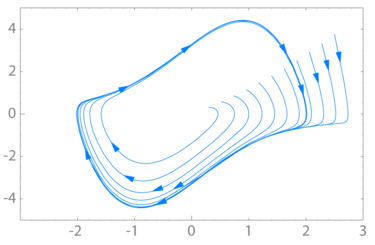
\includegraphics[width = 0.4\textwidth]{figures/375px-VanDerPolPhaseSpace.png}
	\caption{Stable Limit Cycle}
\end{figure}
\subsubsection{Poincaré-Bendixson Criterion}
Consider the system \(\dot x = f(x)\) and let $M$ be a closed bounded subset of the plane such that
\begin{itemize}
	\item $M$ contains no equilibrium points or contains only one equilibrium point such that the Jacobian matrix $[\partial f / \partial x]$ at this point has eigenvalues with positive real parts. (Hence, the equilibrium point is unstable focus or unstable node.)
	\item  Every trajectory starting in $M$ stays in $M$ for all future time.
\end{itemize}
Then, $M$ contains a periodic orbit of $\dot x = f(x)$.
\subsubsection{Benixson Criterion}
If, on a simply connected region ($\mathcal{C}^1$) $D$ of the plane, the expression $\partial f_1 / \partial x_1 + \partial f_2 / \partial x_2$ is not identically zero and does not change sign, then $\dot x= f(x)$ has no periodic orbits lying entirely in D.
\newpage
\section{Lyapunov Stability}
\subsection{Autonomous Systems}
\subsubsection{Stability Principles}
The equilibrium point $x=0$ of $\dot x = f(X)$ is
\begin{itemize}
	\item stable if, for each $\epsilon > 0$, there is a $\delta = \delta(\epsilon) > 0$ such that
	      \begin{equation*}
		      ||x(0)|| < \delta \Rightarrow ||x(t)|| < \epsilon, \quad \forall t \geq 0
	      \end{equation*}
	\item unstable if it is not stable
	\item asymptotically stable if it is stable and $\delta$ can be chosen such that
	      \begin{equation*}
		      ||x(0)|| < \delta \Rightarrow \lim_{t\rightarrow \infty} \; x(t) = 0
	      \end{equation*}
\end{itemize}
\subsubsection{Quadratic Lyapunov Function}
\begin{equation}
	V(x) = \frac{1}{2}x^T Px \textrm{ , } P > 0
\end{equation}
and
\begin{equation}
	\begin{split}
		\frac{d}{dt}V(x) & = \frac{1}{2} x^T P Ax + (x^T PAx)^T \\
		                 & = \frac{1}{2} 2 x^T P\dot x          \\
		                 & = x^T P\dot x
	\end{split}
\end{equation}
\begin{equation}
	\dot V(x) = x^T P\dot x
\end{equation}
In other words
\begin{equation}
	\dot V(x) =
	\begin{bmatrix}
		x_1 \\
		x_2
	\end{bmatrix}^T
	\begin{bmatrix}
		p_{11} & p_{21} \\
		p_{12} & p_{22}
	\end{bmatrix}
	\begin{bmatrix}
		\dot x_1 \\
		\dot x_2
	\end{bmatrix}
\end{equation}
\subsubsection{Asymptotically Stable}
Let $x = 0$ be an equilibrium point and $D \subset R^n$ be a domain
containing $x = 0$. Let $V\::\:D \rightarrow R$ be a continuously differentiable function such
that
\begin{equation}
	V(0) = 0 \quad \textrm{and} \quad V(x) > 0 \; \textrm{in} \; D - \{0\}
\end{equation}
\begin{equation}
	\dot{V}(x) \leq 0 \; \textrm{in} \; D
\end{equation}
Then $x=0$ is stable. Moreover, if
\begin{equation}
	\dot{V}(x) < 0 \; \textrm{in} \; D - \{0\}
\end{equation}
then $x=0$ is asymptotically stable.
\subsubsection{Globally Asymptotic stable}
Let $x=0$ be an equilibrium point or $\dot x = f(x)$. Let $V : \mathbb{R}^n \rightarrow \mathbb{R}$ be a continuously differentiable function such that
\begin{equation*}
	V(0) = 0 \text{  and  } V(x) > 0, \; \forall x \neq 0
\end{equation*}
\begin{equation*}
	||x|| \rightarrow \infty \Rightarrow V(x) \rightarrow \infty
\end{equation*}
\subsubsection{Radially Unbounded Function}
A radially unbounded function is a function $f : \mathbb{R}^n \rightarrow \mathbb{R}$ for which
\begin{equation*}
	||x|| \rightarrow \infty \Rightarrow f(x) \rightarrow \infty
\end{equation*}
Or equivalently
\begin{equation*}
	\forall c > 0 : \exists r > 0 : \forall x \in \mathbb{R}^n : [||x|| > r \Rightarrow f(x) > c]
\end{equation*}
\subsubsection{Region of attraction}
The region of attraction is also called the region of asymptotic stability. The region of attraction may be hard to calculate exactly, but Lyapunov functions can be used to estimate this region.
\\\\
First of all, the region of attraction must satisfy the following: from the definition of asymptotic stability we see that if there is a Lyapunov function that satisfy the condition of asymptotic stability over a domain $\mathbb{D}$ and if $\Omega_c = \{  x \in \mathbb{R}^n | V(x) \leq c\}$ is bounded and contained in $\mathbbD$, then ecery trajectory starting in $\Omega_c$ remains in $\Omega_c$ and approaches the origin as $t \to \infty$
\\\\
Let $x=0$ be an asymptotically stable equilibrium point of the system $\dot x = f(x)$, where $f : \mathbb{D} \to \mathbb{R}^n$ is locally lipschitz and $\mathbb{D} \subset \mathbb{R}^n$ is a domain that contains the origin. Let $t \to \phi(t;x_0)$ be the solution of $\dot x = f(x)$  that starts at initial state $x_0$ at time $t=0$. The region of attraction of the origin, denoted by $R_A$, is defined by
\begin{equation*}
	R_A = \{ x_0 \in \mathbb{D} : \phi(t;x_0) \text{ is defined }\forall t \geq 0 \text{ and } \phi(t;x_0) \to \text{ as } t \to \infty \}
\end{equation*}
I.e. the region of attraction $R_A$ is the set of all points $x_0$ in $\mathbb{D}$ such that the solution of
\begin{equation*}
	\dot x = f(x) \qquad x(0) = x_0
\end{equation*}
is defined for all $t \geq 0$ and converges to the origin as $t \to \infty$.
\begin{frm-ex}[Example of region of attraction]
    \item
	Our domain $\mathbbD$ is defined as
	\begin{equation*}
		\mathbbD = \{ x \in \mathbbR^2 : x_1 + x_2 < 1\}
	\end{equation*}
	where $\dot V(x) < 0$. Our region of attraction is defined as
	\begin{equation*}
		\Omega_c = \{ x \in \mathbbR^2 : V(x) \leq c \}
	\end{equation*}
	where $c < \min(V(x)$ and $x \in \partial c$ (x is on the border of $c$).
	\begin{equation*}
		\begin{split}
			x_1 + x_2 & = 1       \\
			x_1       & = 1 - x_2
		\end{split}
	\end{equation*}
	Then we minimize $V(x)$ with respect of $x_2$
	\begin{equation*}
		\begin{split}
			\min(V(x))_{x_2}\bigg|_{x_1=1-x_2} & = min_{x_2}(\frac{1}{2}((1-x_2)^2+x_2^2)) = 0               \\
			\min_{x_2}(\frac{1}{2}-x_2+x_2^2)  & = \frac{\partial}{\partial x_2} (\frac{1}{2}-x_2+x_2^2) = 0 \\
			-1 + x_2                           & = 0                                                         \\
			x_2                                & = \frac{1}{2} \quad \to \quad x_1 = \frac{1}{2}
		\end{split}
	\end{equation*}
	Further, we must satisfy $c < V(\frac{1}{2}, \frac{1}{2}) = \frac{1}{4}$. We have therefore the following region of attraction
	\begin{equation*}
		\Omega_{\frac{1}{4}} = \{x \in \mathbbR^2 : V(x) \leq \frac{1}{4}\}
	\end{equation*}
\end{frm-ex}
\subsection{The Invariance Principle}
\subsubsection{Invariant Set}
A set $M$ is said to be an invariant set with respect to $\dot x = f(x)$ iff
\begin{equation*}
	x(0) \in M \quad \Rightarrow \quad x(t) \in M, \qquad \forall t \in \mathbb{R}
\end{equation*}
\subsubsection{Positively Invariant Set}
A set $M$ is a positively invariant set with respect to $\dot x = f(x)$ iff
\begin{equation*}
	x(0) \in M \quad \Rightarrow \quad x(t) \in M, \qquad \forall t \geq 0
\end{equation*}
\subsubsection{Lasalle's Theorem}
Lasalle's invariance principle can be used to show the asymptotic stability of an equilibrium point when $\dot V$ is negative semi-definite, $i.e \quad \dot V \leq 0$. $\dot V$ is semidefinite if $\dot V$ is not sticly 0 in origo.
\\\\
Let $\Omega \subset D$ be a compact set that is positively invariant with respect to $\dot x = f(x)$. Let $V\::\:D \rightarrow R$ be a continuously differentiable function such that $\dot V(x) \leq 0$ in $\Omega$. Let $E$ be the set of all points in $\Omega$ where $\dot V(x) = 0$. Let $M$ be the largest invariant set in E. Then every solution starting in $\Omega$ approaches $M$ as $t \rightarrow \infty$.
\begin{figure}[h]
    \centering
	\def\svgwidth{0.5\columnwidth}
    \input{figures/Lasalles.eps_tex}
\end{figure}
\subsubsection{Barbashin Theorem}
Let $x=0$ be an equilibrium point for \[\dot{x} = f(x)\]
Let $V: D \rightarrow R$ be a continuously differentiable positive definite function on a domain $D$ containing the origin $x=0$, such that $\dot V(x) \leq 0$ in $D$. Let $S=\{x \in D\:|\:\dot V(x) = 0\}$ and suppose that no solution can stay identically in $S$, other than the trivial solution $x(t) \equiv 0$. Then, the origin is asymptotically stable.
If a $A$ matrix i Hurwitz, we can conclude asymptotic stability.
\subsubsection{Krasovskii Theorem}
Let \(x = 0\) be an equilibrium point for the system\[\dot{x} = f(x)\]. Let \(V : \mathbb{R}^n \to \mathbb{R}\) be a continuously differentiable, radially unbounded, positive definite function such that \(V(x) \leq 0\) for all \(x \in \mathbb{R}^n\). Let \(S = \{x \in \mathbb{R}^n \,|\, V(x) = 0\}\) and suppose that no solution can stay identically in \(S\), other than the trivial solution \(x(t) = 0\). Then, the origin is globally asymptotically stable.
\subsubsection{Dominating cross-terms}
\paragraph{Completion of squares}
\begin{equation*}
	x_1x_2 \leq \frac{1}{2}(x_1^2 + x_2^2) = \frac{1}{2} ||x||^2_2
\end{equation*}
Another alternative is to write $\dot V$ as $-x^TQx$, where $Q=Q^T$ is positive definite
\paragraph{Youngs inequality}
\begin{equation*}
	xy \leq \epsilon x^2 + \frac{1}{4\epsilon}y^2, \quad \forall \epsilon > 0 \; \forall x,y \in \mathbb{R}
\end{equation*}
\subsubsection{Handling terms with indeterminate sign}
\paragraph{Cauchy-Schwarz Inequality}
\begin{equation*}
	|a_1x_1+a_2x_2+...+a_nx_n|\leq\sqrt{(a_1^2+a_2^2+...+a_n^2}||x||_2
\end{equation*}
\subsection{Linear Systems and Linearization}
\subsubsection{Hurwitz matrix / Stability matrix}
$A$ matrix $A$ is Hurwitz; that is, $Re\{\lambda_i\} < 0$ for all eigenvalues of $A$, if
and only if for any given positive definite symmetric matrix $Q$ there exists a positive
definite symmetric matrix $P$ that satisfies the \textit{Lyapunov equation (\ref{Lyapunov 4.12})}. Moreover,
if $A$ is Hurwitz, then P is the unique solution of (\ref{Lyapunov 4.12}).
\begin{equation}
	PA+A^TP=-Q
	\label{Lyapunov 4.12}
\end{equation}
\\
Another way one can prove asymptotic stability in the origin is by using this symmetric matrix $Q$. We can write $\dot V(x)$ as the following
\begin{equation*}
	\dot V(x) = x^T P \dot x + \dot x^T P x = -x^T Q x
\end{equation*}
If $Q$ is positive definite, we can conclude asymptotic stability at the origin.
\\
\begin{frm-ex}[Example using Hurwitz matrix]
\item
We have the following $\dot V(x)$
\begin{equation*}
	\dot V(x) \leq -x_2^2\left(2 - \frac{1}{4\epsilon}\right) - x_1x_2 - x_1^2(1-\epsilon)
\end{equation*}
We can then formulate the following $Q$ matrix
\begin{equation*}
	Q =
	\begin{bmatrix}
		1 - \epsilon & \frac{1}{2}              \\
		\frac{1}{2}  & 2 - \frac{1}{4 \epsilon}
	\end{bmatrix}
\end{equation*}
To ensure that $Q$ is positive definite we can evaluate the principle of minors
\begin{equation*}
	(1 - \epsilon) \left( w - \frac{1}{4 \epsilon} \right) - \frac{1}{4} > 0
\end{equation*}
while $(1 - \epsilon) > 0$. We can solve the las inequality, and $\epsilon$ must satisfy
\begin{equation*}
	\frac{2 - \sqrt{2}}{4} < \epsilon < \frac{2 + \sqrt{2}}{4}
\end{equation*}
to ensure that the origin is asymptotically stable.
\end{frm-ex}

\subsubsection{Indirect Method}
Let \(x = 0\) be an equilibrium point for the nonlinear system
\[
	\dot{x} = f(x)
\]
where \(f : D \to \mathbb{R}^n\) is continuously differentiable and \(D\) is a neighborhood of the origin. Let
\[
	A = \frac{\partial f}{\partial x_i}\bigg|_{x=0}
\]
Then,
\begin{enumerate}
	\item The origin is asymptotically stable if \(\text{Re}(\lambda_i) < 0\) for all eigenvalues \(\lambda_i\) of \(A\).
	\item The origin is unstable if \(\text{Re}(\lambda_i) > 0\) for one or more of the eigenvalues \(\lambda_i\) of \(A\).
\end{enumerate}
\subsection{Comparison Functions}
\subsubsection{Class $\mathcal{K}$ and Class $\mathcal{K}_{\infty}$ Definitions}
A continuous function \(\alpha : [0, a) \to [0, \infty)\) is said to belong to class \(\mathcal{K}\) if it is strictly increasing and \(\alpha(0) = 0\). It is said to belong to class \(\mathcal{K}_\infty\) if \(a = \infty\) and \(\alpha(r) \to \infty\) as \(r \to \infty\).
\subsubsection{Class $\mathcal{K}\mathcal{L}$ Definition}
A continuous function \(\beta : [0, a) \times [0, \infty) \to [0, \infty)\) is said to belong to class \(\mathcal{K}\mathcal{L}\) if, for each fixed $s$, the mapping $\beta(r,s)$ belongs to $\mathcal{K}$ with respect to $r$ and, for each fixed $r$, the mapping $\beta(r,s)$ is decreasing with respect to $s$ and \(\beta(r,s) \to \infty\) as \(s \to \infty\).
%\end{multicols*}
\subsubsection{Class $\mathcal{K}$, $\mathcal{K}_{\infty}$ and $\mathcal{K}\mathcal{L}$ Rules}
Let $\alpha_1$ and $\alpha_2$ be class $\mathcal{K}$ functions on $[0,a),\alpha_3$ and $\alpha_4$ be class $\mathcal{K}-\infty$
\begin{frm-ex}[Class $\mathcal{K}$]

\item $\alpha(r) = \tan^{-1}$ is strictly increasing since $\dot \alpha(r)=\frac{1}{(1+r^2)}>0$. It belongs to calss $\mathcal{K}$, but not to class $\mathcal{K}_{\infty}$ since $\lim_{r \rightarrow \infty} \alpha(r) = \frac{\pi}{2} < \infty$.
\end{frm-ex}
\begin{frm-ex}[Class $\mathcal{K}\mathcal{L}$]
\item $\beta(r,s) = \frac{r}{(ksr+1)}$ , for any positive real number $k$, is strictly increasing in $r$ since
\begin{equation*}
	\frac{\partial \beta}{\partial r} = \frac{ks}{(ksr+1)^2} > 0
\end{equation*}
and stricly decreasuing in $s$ since
\begin{equation*}
	\frac{\partial \beta}{\partial s} = \frac{-kr^2}{(ksr+1)^2} < 0
\end{equation*}
Moreover $\beta(r,s) \rightarrow 0 \text{ as } s \rightarrow \infty$
\end{frm-ex}
\subsubsection{Introducing class $\mathcal{K}$ functions in Lyapunov's stability theorem}
Let $\alpha_1$ and $\alpha_2$ be class $\mathcal{K}$ functions on $[0, a), \alpha_3$ and $\alpha_4$ be class $\mathcal{K}_{\infty}$ functions, and $\beta$ be a class $\mathcal{K} \mathcal{L}$ function. Denote the inverse of $\alpha_i$ by $\alpha_i^{-1}$. Then,
\begin{itemize}
    \item $\alpha_1^{-1}$ is defined on $\left[0, \alpha_1(a)\right)$ and belongs to class $\mathcal{K}$.
    \item $\alpha_3^{-1}$ is defined on $[0, \infty)$ and belongs to class $\mathcal{K}_{\infty}$.
    \item $\alpha_1 \circ \alpha_2$ belongs to class $\mathcal{K}$.
    \item $\alpha_3 \circ \alpha_4$ belongs to class $\mathcal{K}_{\infty}$.
    \item $\sigma(r, s)=\alpha_1\left(\beta\left(\alpha_2(r), s\right)\right)$ belongs to class $\mathcal{K} \mathcal{L}$.
\end{itemize}
Class $\mathcal{K}$ and class $\mathcal{K} \mathcal{L}$ functions enter into Lyapunov analysis through the next subsections
\subsubsection{Lyapanovs analysis with Class $\mathcal{K}$ functions}
Let $V: D \rightarrow R$ be a continuous positive definite function defined on a domain $D \subset R^n$ that contains the origin. Let $B_r \subset D$ for some $r>0$. Then, there exist class $\mathcal{K}$ functions $\alpha_1$ and $\alpha_2$, defined on $[0, r]$, such that
\[
\alpha_1(\|x\|) \leq V(x) \leq \alpha_2(\|x\|)
\]
for all $x \in B_r$. If $D=R^n$, the functions $\alpha_1$ and $\alpha_2$ will be defined on $[0, \infty)$ and the foregoing inequality will hold for all $x \in R^n$. Moreover, if $V(x)$ is radially unbounded, then $\alpha_1$ and $\alpha_2$ can be chosen to belong to class $\mathcal{K}_{\infty}$.
\subsubsection{Lyapanovs analysis with Class $\mathcal{K} \mathcal{L}$ functions}
Consider the scalar autonomous differential equation
$$
\dot{y}=-\alpha(y), \quad y\left(t_0\right)=y_0
$$
where $\alpha$ is a locally Lipschitz class $\mathcal{K}$ function defined on $[0, a)$. For all $0 \leq y_0<a$, this equation has a unique solution $y(t)$ defined for all $t \geq t_0$. Moreover,
$$
y(t)=\sigma\left(y_0, t-t_0\right)
$$
where $\sigma$ is a class $\mathcal{K} \mathcal{L}$ function defined on $[0, a) \times[0, \infty)$.
\subsection{Nonautonomous Systems}
Throughout this section we will consider the following Nonautonomous system
\begin{equation*}
    \dot x = f(t,x)
    \label{Nonautonomous system}
\end{equation*}
\subsubsection{Stability definitions}
The equilibrium point $x=0$ of \ref{Nonautonomous system} is
\begin{itemize}
    \item stable if, for each $\varepsilon>0$, there is $\delta=\delta\left(\varepsilon, t_0\right)>0$ such that
$$
\left\|x\left(t_0\right)\right\|<\delta \Rightarrow\|x(t)\|<\varepsilon, \quad \forall t \geq t_0 \geq 0
$$
    \item uniformly stable if, for each $\varepsilon>0$, there is $\delta=\delta(\varepsilon)>0$, independent of $t_0$, such that (4.16) is satisfied.
    \item unstable if it is not stable.
    \item asymptotically stable if it is stable and there is a positive constant $c=c\left(t_0\right)$ such that $x(t) \rightarrow 0$ as $t \rightarrow \infty$, for all $\left\|x\left(t_0\right)\right\|<c$.
	\item Asymptotically stable (AS) if
	\subitem it is stable
	\subitem there exists $c>0$ s.t. for all $t_0 \geq 0$ and $\eta>0$, there exists $T\left(t_0, \eta\right)>0$ satisfying
	$$
	\left\|x\left(t_0\right)\right\| \leq c \Longrightarrow\|x(t)\| \leq \eta \quad \forall t \geq t_0+T\left(t_0, \eta\right)
	$$
	\item Uniformly asymptotically stable (UAS) if
	\subitem it is uniformly stable (US)
	\subitem there exists $c>0$ s.t. for all $t_0 \geq 0$ and $\eta>0$, there exists $T(\eta)>0$ satisfying
	$$
	\left\|x\left(t_0\right)\right\| \leq c \Longrightarrow\|x(t)\| \leq \eta \quad \forall t \geq t_0+T(\eta)
	$$
	
	\item Globally uniformly asymptotically stable (GUAS) if
	\subitem it is globally uniformly stable (GUS)
	\subitem for all $\eta, c>0$ and $t_0 \geq 0$ there exists $T(\eta, c)>0$ s.t.
	$$
	\left\|x\left(t_0\right)\right\| \leq c \Longrightarrow\|x(t)\| \leq \eta \quad \forall t \geq t_0+T(\eta, c)
	$$
\end{itemize}
\subsubsection{Equlibirum Points}
$x^* \in \mathbb{R}^n$ is an equilibrium point of $\dot x = f(t,x)$ if $f(t,x^*) = 0$ for all $t \geq 0$.
\begin{frm-ex}[Example of equilibrium point]
	\item $\dot x = -\frac{a(t)x}{1+x^2}$ has the equilibrium point $x^* = 0$. We can see this by evaluating $f(t,x^*)$
	\item $\dot x = -\frac{a(t)}{1+x^2}+b(t)$ where $b(t) \neq 0 \; \forall t$ has no equilibrium points
\end{frm-ex}
\subsubsection{Stability definitions with $\mathcal{K}$ and $\mathcal{KL}$ classes}
For $\dot x = f(t,x)$, the equilibrium point $x^* = 0$ is
\begin{itemize}
	\item Uniformly stable (US) if $\exists \alpha \in \mathcal{K}, \exists c > 0$ such theoremseparator
			\begin{equation*}
				\| x(t) \| \leq \alpha(\|x(t_0\|)) \quad \forall t \geq t_0, \quad \|x(t_0)\| \leq c, \quad \forall t_0 \geq 0
			\end{equation*}
	\item globally uniformly stable (GUS) if $\exists \alpha \in \mathcal{K}_{\infty}$ such that
	\begin{equation*}
		\| x(t) \| \leq \alpha(\|x(t_0\|)) \quad \forall t \geq t_0, \quad \forall t_0 \geq 0
	\end{equation*}
	\item exponentially stable if $\exists c,k, \lambda > 0$
	\begin{equation*}
		\|x(t)\| \leq k \|x(t_0)\|e^{-\lambda(t-t_0)} \qquad t \geq t_0 \geq 0, qquad \|x(t_0)\| < c
	\end{equation*}
	\item globally exponentially stable if $\exists k, \lambda > 0$
	\begin{equation*}
		\|x(t)\| \leq k \|x(t_0)\|e^{-\lambda(t-t_0)} \qquad t \geq t_0 \geq 0, qquad \forall x(t_0)
	\end{equation*}
\end{itemize}
\subsubsection{Time-varying Lyapunov function candidates}
$V(t,x)$ is positive definite if
\begin{equation*}
	\begin{rcases}
		V(t,0) = 0 \\
		V(t,x) \geq W_1(x)
	\end{rcases}
	\forall t \geq 0 \text{, for some positive definitie function } W_1(x)
\end{equation*}
and
\begin{itemize}
	\item $(t,x) \rightarrow V(t,x)$ is positive semidefinite if $x \rightarrow	W_1(x)$ positive semidefinite
	\item $(t,x) \rightarrow V(t,x)$ is radially unbounded if $x \rightarrow	W_1(x)$ radially unbounded
\end{itemize}
$V(t,x)$ is decresent if
\begin{equation*}
	\begin{rcases}
		V(t,0) = 0 \\
		V(t,x) \leq W_2(x)
	\end{rcases}
	\forall t \geq 0, \text{ for some positive definite function } W_2(x)
\end{equation*}
\begin{figure}[h]
	\centering
	\def\svgwidth{0.5\columnwidth}
    \input{figures/Lyapunov_function.eps_tex}
\end{figure}
\subsubsection{Lyapunov theorem: Uniformal Stability}
If there exitst a function $V(t,x):[0, \infty) \times \mathbbD \rightarrow \mathbbR$ and $W_i: \mathbb{D} \rightarrow \mathbb{R}$ continuous positive definite such that
\begin{enumerate}[i)]
	\item $V \text{ is } C^1$
	\item $W_1(x) \leq V(t,x) \leq W_2(x) \qquad \forall (t,x) \in [0, \infty) \times \mathbb{D}$
	\item $\dot V(t,x) \leq 0 \qquad \forall (t,x) \in [0, \infty) \times \mathbb{D}$
\end{enumerate}
then $x=0$ is uniformly stable.
\subsubsection{Lyapunov theorem: Asymptotical Stability}
If there exitst a function $V(t,x):[0, \infty) \times \mathbbD \rightarrow \mathbbR$ and $W_i: \mathbb{D} \rightarrow \mathbb{R}$ continuous positive definite such that
\begin{enumerate}[i)]
	\item $V \text{ is } C^1$
	\item $W_1(x) \leq V(t,x) \leq W_2(x) \qquad \forall (t,x) \in [0, \infty) \times \mathbb{D}$
	\item $\dot V(t,x) \leq -W_3(x) \qquad \forall (t,x) \in [0, \infty) \times \mathbb{D}$
\end{enumerate}
then $x=0$ is asymptotically stable.
\subsubsection{Lyapunov theorem: Global Uniformly Asymptotical Stability}
If there exitst a function $V(t,x):[0, \infty) \times \mathbb{R}^2 \rightarrow \mathbbR$ and $W_i: \mathbb{R}^2 \rightarrow \mathbb{R}$ continuous positive definite such that
\begin{enumerate}[i)]
	\item $V \text{ is } C^1$
	\item $W_1(x) \leq V(t,x) \leq W_2(x) \qquad \forall (t,x) \in [0, \infty) \times \mathbb{D}$
	\item $\dot V(t,x) \leq -W_3(x) \qquad \forall (t,x) \in [0, \infty) \times \mathbb{D}$
	\item $W_1$ is radially unbounded
\end{enumerate}
then $x=0$ is globally asymptotically stable.
\subsubsection{Lyapunov theorem: Exponential Stability}
If there exist a function $V(t,x):[0, \infty) \times \mathbb{D} \rightarrow \mathbbR$ and constants $a, k_1, k_2, k_3 > 0$ such that
\begin{enumerate}[i)]
	\item $V \text{ is } C^1$
	\item $k_1 \|x\|^a \leq V(t,x) \leq k_2 \|x\|^a \qquad \forall (t,x) \in [0, \infty) \times \mathbb{D}$
	\item $\dot V(t,x) \leq -k_3 \|x\|^a \qquad \forall (t,x) \in [0, \infty) \times \mathbb{D}$
\end{enumerate}
then $x=0$ is exponentially stable.
\subsubsection{Barbalat's Lemma}
If there exist functions $V:[0, \infty) \times \mathbb{R}^n \rightarrow \mathbb{R}^n, W_i: \mathbb{R}^n \rightarrow \mathbb{R}$ continuous positive definite and radially unbounded and $W: \mathbb{R}^n \rightarrow \mathbb{R}^n C^1$ and positive semidefinite satisfying
\begin{enumerate}[i)]
	\item $V$ is $C^1$
	\item $W_1(x) \leq V(t, x) \leq W_2(x) \quad \forall(t, x) \in[0, \infty) \times \mathbb{R}^n$
	\item $\dot{V}(t, x) \leq-W(x) \quad \forall(t, x) \in[0, \infty) \times \mathbb{R}^n$
	\item for every $k>0$ there exists $c>0$ s.t. $\|x\| \leq k \Longrightarrow|\dot{W}(t, x)| \leq c$ for all $t \geq 0$
\end{enumerate}
then the origin is globally uniformly stable and all solutions approach $E=\left\{x \in \mathbb{R}^n: W(x)=0\right\}$.
\subsubsection{LaSalles-Yokishawa Theorem}
$\dot x = f(t, x)$ where $f:[0, \infty) \times \mathbb{D} \rightarrow \mathbb{R}^n$ is piecewise continuous locally Lipschitz in $x$ and $x=0$ is an eq.point.
\\\\
If there exist functions $V:[0, \infty) \times \mathbb{D} \rightarrow \mathbb{R}, W_i: \mathbb{D} \rightarrow \mathbb{R}$ continuous positive definite, $W: \mathbb{D} \rightarrow \mathbb{R}$ continuous positive semidefinite, such that
\begin{enumerate}[i)]
	\item $V$ is $C^1$
	\item $W_1(x) \leq V(t, x) \leq W_2(x) \quad \forall(t, x) \in[0, \infty) \times \mathbb{D}$
	\item $\dot{V}(t, x) \leq-W(x) \quad \forall(t, x) \in[0, \infty) \times \mathbb{D}$
	\item for every $k>0$ there exists $r>0$ s.t. $\|x\| \leq k \Longrightarrow\|f(t, x)\| \leq r$ for all $t \geq 0$ 
\end{enumerate}
then the origin is uniformly stable, and $\exists c>0$ such that all solutions with $\left\|x\left(t_0\right)\right\|<c$ approach $E=\{x \in \mathbb{D}: W(x)=0\}$
\subsubsection{Global LaSalles-Yokishawa Theorem}
$\dot x = f(t, x)$ where $f:[0, \infty) \times \mathbb{D} \rightarrow \mathbb{R}^n$ is piecewise continuous locally Lipschitz in $x$ and $x=0$ is an eq.point.
\\\\
If there exist functions $V:[0, \infty) \times \mathbb{R}^n \rightarrow \mathbb{R}, W_i: \mathbb{R}^n \rightarrow \mathbb{R}$ continuous positive definite and radially unbounded, $W: \mathbb{R}^n \rightarrow \mathbb{R}$ continuous positive semidefinit
\begin{enumerate}[i)]
	\item $V$ is $C^1$
	\item $W_1(x) \leq V(t, x) \leq W_2(x) \quad \forall(t, x) \in[0, \infty) \times \mathbb{R}^n$
	\item $\dot{V}(t, x) \leq-W(x) \quad \forall(t, x) \in[0, \infty) \times \mathbb{R}^n$
	\item for every $k>0$ there exists $r>0$ s.t. $\|x\| \leq k \Longrightarrow\|f(t, x)\| \leq r$ for all $t \geq 0$
\end{enumerate}
then the origin is globally uniformly stable and all solutions approach $E=\left\{x \in \mathbb{R}^n: W(x)=0\right\}$+
Test 123
\end{document}
